\chapter{Data Quality}
Various projects today is focused on gathering data and analysing it. The gathered data is used for obtaining behaviours, habits and properties of the observed objects. This is done by using powerful statistical leaning algorithms, that are able to deduce these properties from the data. This approach is called data driven development, since the success is mainly determined by the data and not the algorithm. 

When data is the central role of the system, the quality of the data are very important. Poor data can lead to wrong assumptions, and have a negative effect on the application. Choosing the correct dataset is therefore a key factor \cite{RefWorks:3}. Looking at the quality of the data can help you chose what dataset to use. Data quality can be described many ways, one of the more formal is from the ISO 8402 standard that describes quality as: 

\begin{adjustwidth}{2.5em}{2.5em}
\emph{"The totality of characteristics of an entity that bear upon its ability of satisfy stated and implied needs"} \cite{RefWorks:5}.
\end{adjustwidth}

This indicate that data quality is something that is very depended on the intended application, and is therefore hard to generalize. 

Quality of data is a subject that is gaining more and more attention due to the fact that the quantity of data available is larger than ever before. This forces researchers to choose between datasets, and a notion of quality in the dataset can help them choose. The heavy growth in available data is a result of projects that are moving data gathering from controlled labs, to the public. Many of these projects is citizen science projects, where it is the citizens who collect the data, and not the researchers \cite{RefWorks:2}. This enables researchers to gather enormous amount of data, but they are no longer in control of the conditions the data is collected in, which introduces errors and other quality decreasing factors. 

\section{Quality Criteria}
It is not uncommon that different areas of of research has its own quality criteria. This is due to the fact that quality is a very domain specific subject. One of the areas that have been dealing with citizen data for many years is the Geographic information area, that are used for maps, weather prediction and climate research. They have come up with several ways of describing quality in spatial data \cite{RefWorks:7}. Method for defining quality in time series data have also been developed  \cite{RefWorks:6}. 

One of the things all the methods have in common is trying to look at the completeness of the data. Some of the most low level criteria is the sample availability. The sample availability describes how many samples there is collected in relation to the expected collection amount, and look at how the samples is distributed in the measurement period.  


\section{Quality In SmartHG Citizen Data}
As a part of the SmartHG project 25 households have been equipped with meters on selected appliances and the main meter. The data collected from this experiment are prone with errors due to malfunctioning test equipment or unexpected interference from the resident which have resulted in offline measurement equipment for periods of time. 

The SmartHG data is intended for appliance recognition, and the quality must be assessed with this in mind. First a completeness analysis is done on the data, by analysing the sample availability quality of the data. 

The analysis is done in small segments on one hour. The quality of a given meter in a given hour is defined as the ratio of observed samples over the expected samples. 
\begin{gather}
		N_{max}^{(m,T)} = \floor{ \frac{(T_{P}-\phi_{start}^{(m,T)})}{T_s^{(m)}}} + 1 \label{EQ:NMAX} \\
		q^{(m,T)} = \frac{N_{observed}^{(m,T)}}{ N_{max}^{(m,T)} } \label{EQ:QMT}
\end{gather}
As shown on equation \ref{EQ:NMAX} is the maximum number of samples for a meter $m$ in the period $T$ calculated by taking the period time $T_P$, corrected with the sample phase $\phi_{start}$ for the given period, and dividing it with the sample time $T_s$. The quality of the meter is calculated as the ratio of observed samples in the timeslot $T$ to the maximum samples, shown in equation \ref{EQ:QMT}. 

To find the quality of a house in a given period $T$, that have a set of meters $M$, we take the mean value of all the meter quality's, as shown in equitation \ref{EQ:HQT}.  
\begin{equation}
	\mu_{q^{(M,T)}} = \frac{1}{\mathbf{card}(M)} \sum_{m \in M} q^{(m,T)}
	\label{EQ:HQT}
\end{equation}
Each house have a quality vector $Q$, with the house quality found whit a period $T_P$ on one hour. This have been done from March $t_{start}$ to October $t_{end}$. 
\begin{equation}
	Q^{(M,t_{start},t_{end} )} = \{ \mu_{q^{(M,T)}} | T \in \{t_{start}, t_{start}+T_p,t_{start}+2 \times T_p, ... , t_{end}  \} \}
	\label{EQ:HQV}
\end{equation}
This is shown in equation \ref{EQ:HQV} where M is a set of the meters in a given house. This can be graphically shown on the figure \ref{fig:SmartHGQuality} where all the houses $Q$ vectors is shown. The color is a gradient running from light green for the best quality to red for bad quality.
\begin{figure}[H]
\centering
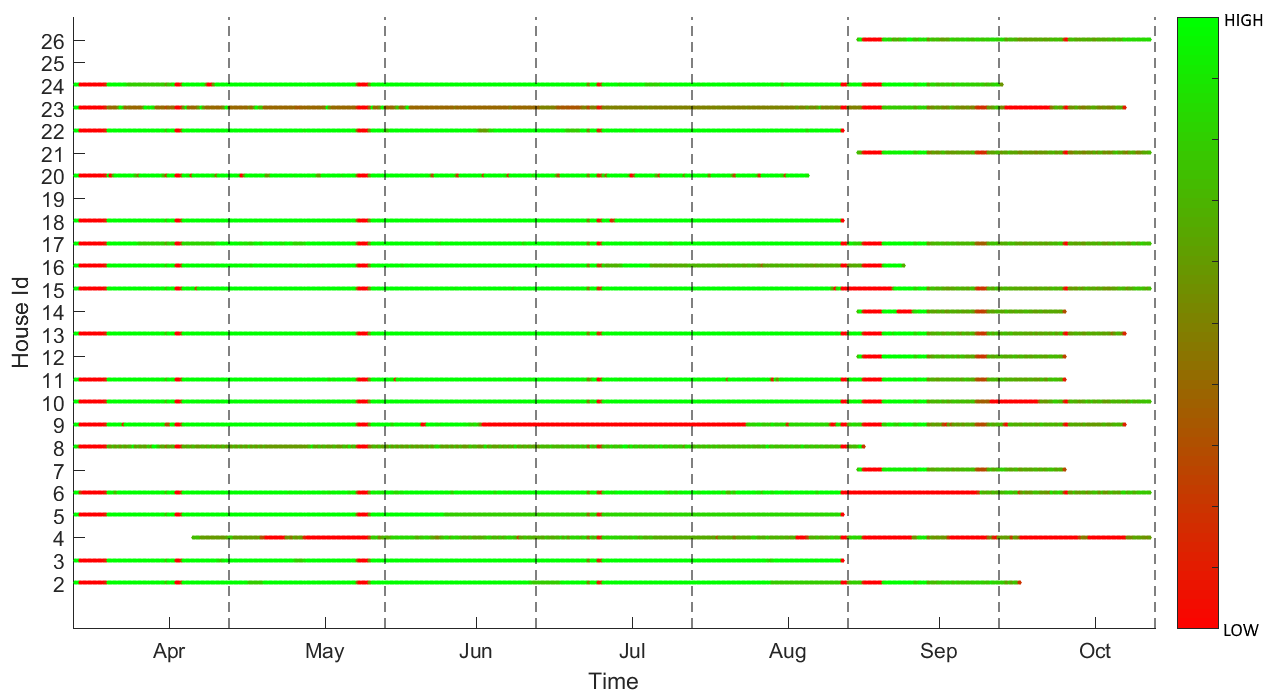
\includegraphics[width=1\textwidth]{billeder/QualityBig.png}
\caption{Quality of houses in SmartHG project}
\label{fig:SmartHGQuality}
\end{figure} 
Since the data is intended for appliance recognition it is also of interest where in the data there is activity, and where there is not happening anything. We define activity as area in the data where $f(x) \neq f(x+1) $. The standard deviation of a area is a good metric to indicate this behaviour. This is shown on figure \ref{fig:ActivityMap} where green is high activity and red is non activity. 
\begin{figure}[H]
\centering
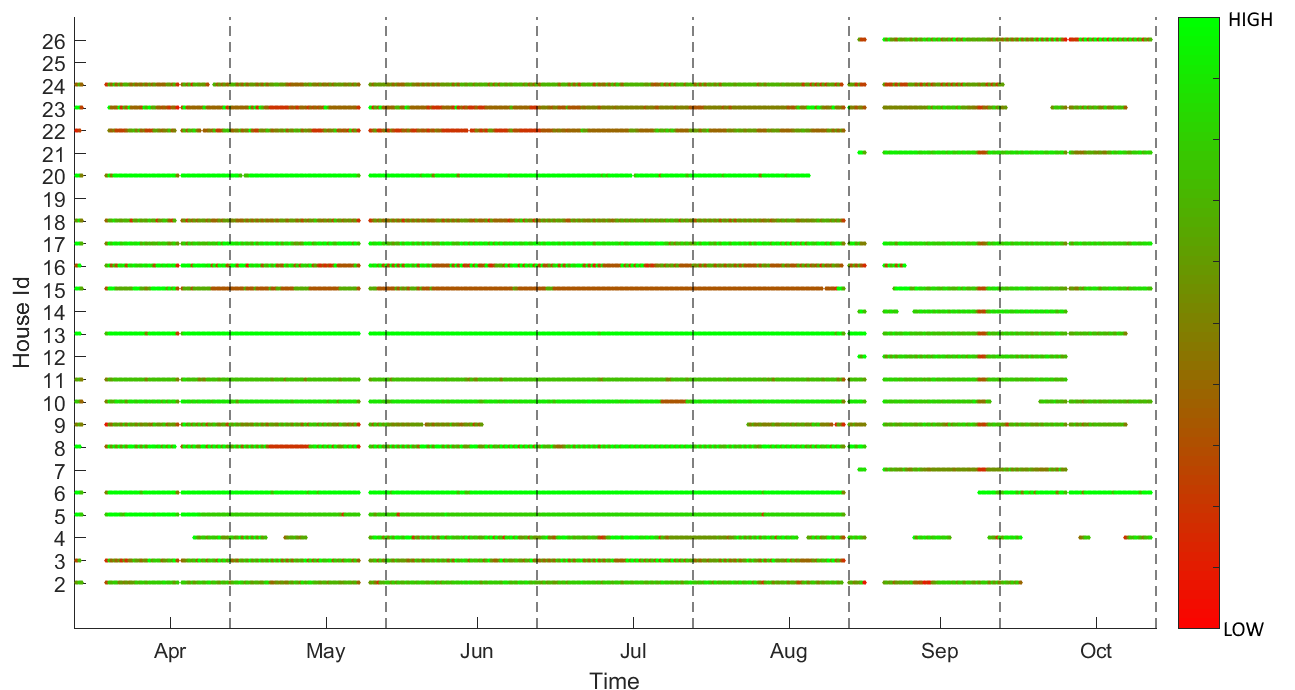
\includegraphics[width=1\textwidth]{billeder/ActivityBig.png}
\caption{Activity of houses in SmartHG project}
\label{fig:ActivityMap}
\end{figure}

\section{Related Work}
Data Quality is a area that recently have become a hot topic, due to the wast quantity of data. Many researchers strive to make tools that better can analyse data quality in different areas. In the area of spatial data is a \emph{"Quality and Workflow tool"} being developed by the University of Wageningen \citep{RefWorks:8}. The objective is to help researchers select the best suited data for a given data driven project. It does this by looking at different quality criteria, given by the user or found in standards for spatial data. 

In bioinformatics is a tool named QCScreen developed to help create better dataset to metabolomics studies. In metabolomics studies is dataset often created by joining information from several different experiments of various quality. By using tools that can check the data quality and consistency to determine if a dataset is suitable for further processing, they are able to greatly improve the test results \citep{RefWorks:9}.
 
In the article \emph{Taking a big Data approach to data quality in a citizen science project}\citep{RefWorks:2} they talk about how quality assessment can be used to rate the 
believe on your data, and how to improve data collected in citizen science. The project focuses on bird observations, done by users on their smartphones. They improve the quality by disallowing the user to send incomplete datasets to the database, and in this way forcing the user to only deliver high quality information. They then cross check the information whit information from people in the same area, to see if it varies greatly. 

Common for all the methods above is that they deal whit completeness of the signal.